%%%%%%%%%%%%%%%%%%%%%%%%%%%%%%%%%%%%%%%%%
% NIWeek 2014 Poster by T. Reveyrand
% www.microwave.fr
% http://www.microwave.fr/LaTeX.html
% ---------------------------------------
% 
% Original template created by:
% Brian Amberg (baposter@brian-amberg.de)
%
% This template has been downloaded from:
% http://www.LaTeXTemplates.com
%
% License:
% CC BY-NC-SA 3.0 (http://creativecommons.org/licenses/by-nc-sa/3.0/)
%
%%%%%%%%%%%%%%%%%%%%%%%%%%%%%%%%%%%%%%%%%

%----------------------------------------------------------------------------------------
%	PACKAGES AND OTHER DOCUMENT CONFIGURATIONS
%----------------------------------------------------------------------------------------

\documentclass[a0paper,portrait]{baposter}

\usepackage[font=small,labelfont=bf]{caption} % Required for specifying captions to tables and figures
\usepackage{booktabs} % Horizontal rules in tables
\usepackage{relsize} % Used for making text smaller in some places

\usepackage{amsmath,amsfonts,amssymb,amsthm} % Math packages
\usepackage{eqparbox}

\usepackage{textcomp}

\graphicspath{{figures/}} % Directory in which figures are stored

 \definecolor{bordercol}{RGB}{40,40,40} % Border color of content boxes
 \definecolor{headercol1}{RGB}{186,215,230} % Background color for the header in the content boxes (left side)
 \definecolor{headercol2}{RGB}{120,120,120} % Background color for the header in the content boxes (right side)
 \definecolor{headerfontcol}{RGB}{0,0,0} % Text color for the header text in the content boxes
 \definecolor{boxcolor}{RGB}{210,235,250} % Background color for the content in the content boxes


\begin{document}

\background{ % Set the background to an image (background.pdf)
\begin{tikzpicture}[remember picture,overlay]
\draw (current page.north west)+(-2em,2em) node[anchor=north west]
{\includegraphics[height=1.1\textheight]{background}};
\end{tikzpicture}
}

\begin{poster}{
grid=false,
borderColor=bordercol, % Border color of content boxes
headerColorOne=headercol1, % Background color for the header in the content boxes (left side)
headerColorTwo=headercol2, % Background color for the header in the content boxes (right side)
headerFontColor=headerfontcol, % Text color for the header text in the content boxes
boxColorOne=boxcolor, % Background color for the content in the content boxes
headershape=roundedright, % Specify the rounded corner in the content box headers
headerfont=\Large\sf\bf, % Font modifiers for the text in the content box headers
textborder=rectangle,
background=user,
headerborder=open, % Change to closed for a line under the content box headers
boxshade=plain
}

%
%----------------------------------------------------------------------------------------
%	TITLE AND AUTHOR NAME
%----------------------------------------------------------------------------------------
%
{ \bf  \huge {An Autocompletion Algorithm using Recurrent Neural Networks} } % Poster title
{\vspace{0.3em} \smaller Marvin Klaus$^1$, Daniela Schacherer$^2$, Sebastian Bek$^3$  \\  % Author names
  
\smaller $^1$\it {Heidelberg University, M.Sc. Applied Computer Science} \\ $^2$\it{Heidelberg University, M.Sc. Applied Computer Science} \\ $^3$\it{Heidelberg University, M.Sc. Applied Computer Science} % Author email addresses  
  
 } % Author email addresses
%{\includegraphics[scale=0.45]{NI.jpg}} % University/lab logo

%----------------------------------------------------------------------------------------
%	INTRODUCTION
%----------------------------------------------------------------------------------------
\headerbox{Introduction}{name=introduction,column=0,row=0, span=3}{
A classical feedforward network expects data that are independent from each other as well as idenpendently and identically distributed. It follows that there is also no relation between the current and the previous output of the network. However there are some scenarios where the previous output is needed in order to get the new output. This is for example the case when dealing with sequences like text, genomes or numerical time series data. Here a meaningful prediction can only be made based on the current and one or multiple previous outputs.
In such cases \textbf{recurrent neural networks} (RNN) are the method of choice.

\begin{center}
	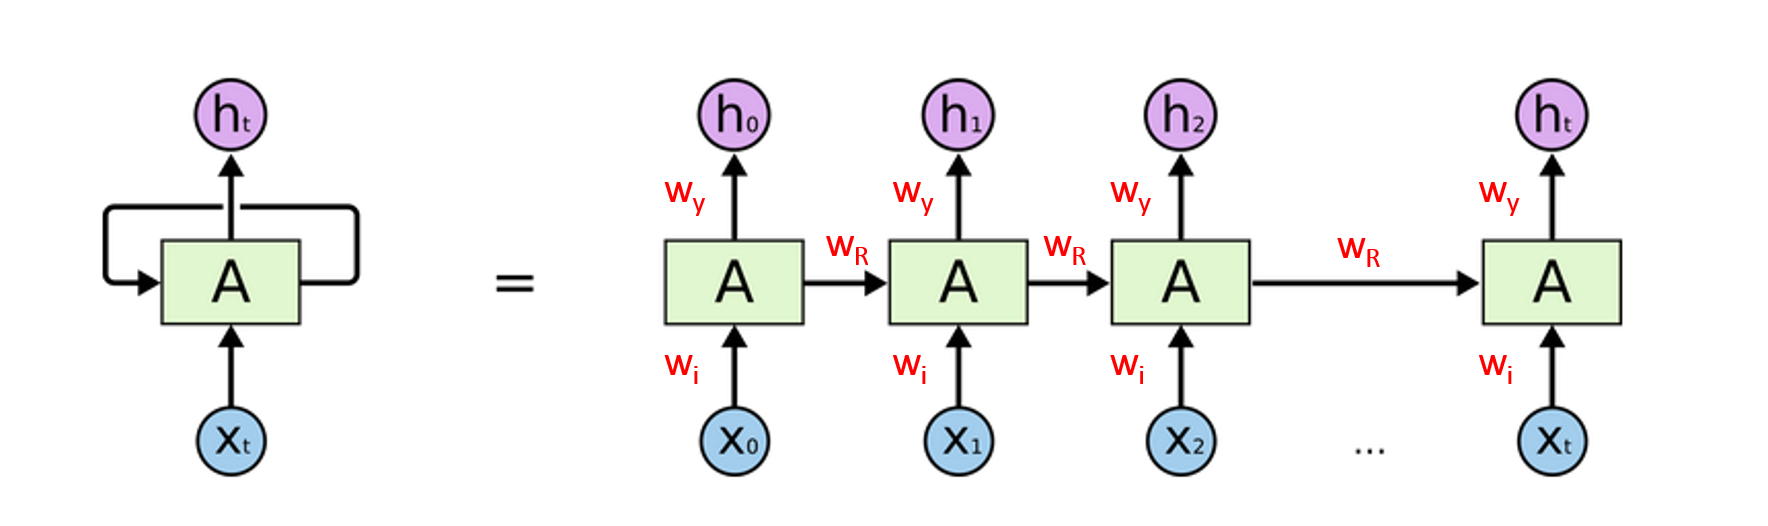
\includegraphics[width=0.35\linewidth]{rnn2}
\end{center}

Hereby each of the unrolled network states $A$ receives the current input $x_t$ as well as the input at time $t-1$ and computes the ouput considering both.

\textbf{Long term dependencies}: \\
RNNs like the one above can memorize the information from the timepoint directly before the current time. But there are also situations where the information from even earlier is needed for the prediction, which is where \textbf{long short term memory networks (LSTMs)} come into play.

}



%----------------------------------------------------------------------------------------
%	CALIBRATION
%----------------------------------------------------------------------------------------
\headerbox{RESULTS}{name=calibration,column=0,below=introduction}{
\textbf{Data Model}


\textbf{System}


}

%----------------------------------------------------------------------------------------
%	OTHER INSTRUMENTATION
%----------------------------------------------------------------------------------------
\headerbox{LSTM Architecture}{name=instruments,span=2,column=1,row=1, below=introduction}{ % To reduce this block to 1 column width, remove 'span=2'
{
For our purpose we decided to use long short term memory networks (LSTMs). In comparison to simple RNNs, LSTMs have a more complex repeating module each consisting of four interacting layers. The horizontal line passing the module is the central part of an LSTM, also called the cell state $C$. There are three gates that allow to introduce or remove information from the cell state: \\

\begin{minipage}[c]{0.6\textwidth}
\begin{itemize}
\item What to forget: $f_t = \sigma(W_f \cdot [h_{t-1}, x_t] + b_f)$
	\item Values to add: $\tilde{C}_t = tanh(W_C \cdot [h_{t-1}, x_t] + b_C)$
	\item What to add: $i_t = \sigma(W_i \cdot [h_{t-1}, x_t] + b_i)$
	\item The new cell state: $C_t = f_t \cdot C_{t-1} + i_t \cdot \tilde{C}_t$
	\item Module output $h_t$: \\
	$o_t = \sigma(W_o \cdot [h_{t-1}, x_t] + b_o)$ \\
	$h_t = o_t \cdot tanh(C_t)$
\end{itemize}
\end{minipage}
\hfill
\begin{minipage}[l]{0.4\textwidth}
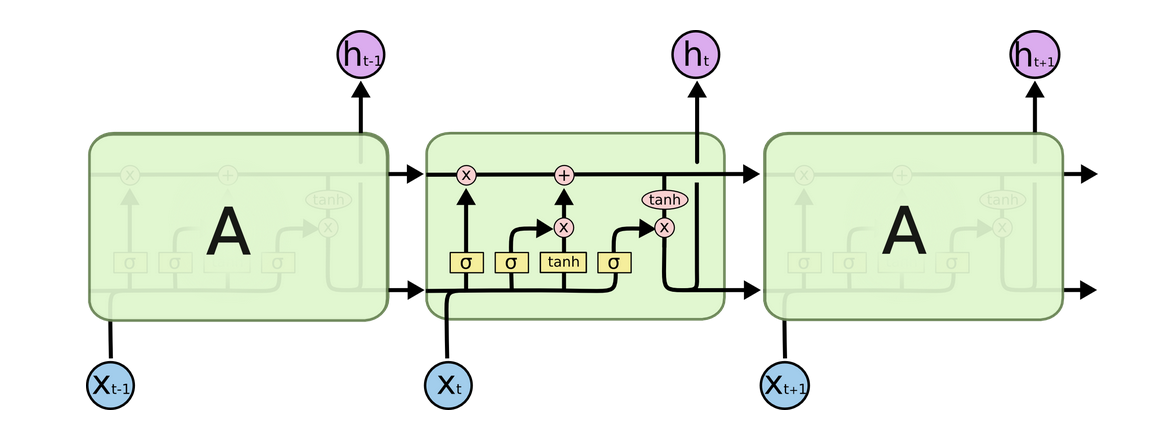
\includegraphics[width=\textwidth]{lstm}
\end{minipage}
}
}


%----------------------------------------------------------------------------------------
%	MIXER vs. SAMPLERS
%----------------------------------------------------------------------------------------
%\headerbox{Receiver: Mixer vs. Sampler}{name=receiver,span=2,column=1,row=1, below=instruments}{
%\begin{center}
%\includegraphics[width=1\linewidth]{RECEIVER.pdf}
%\end{center}
%}


%----------------------------------------------------------------------------------------
%	MEASUREMENT SETUP
%----------------------------------------------------------------------------------------
\headerbox{Requirements and Concept}{name=application,span=2,column=1,below=instruments}{ 
\textbf{Requirements} \\
We used the programming language python and pytorch as the framework to implement our neural network.\\ 

\textbf{Concept}\\
We used xxx as training set for our model. We decided to use a relatively small training set that allows training on a CPU. Our workflow consists of the following steps:
\begin{itemize}
	\item \textbf{Data preprocessing and construction of the training set}: We splitted our text into slices of a predefined length (here: 30 characters) spacing the sequences by a predefined offset (here: 4 characters). The data were than converted into an One-Hot encoding.
	\item \textbf{Training of the RNN}: For training we used an RNN consisting of an LSTM architecture with 128 neurons, followed by a fully connected layer with as many neurons as unique characters exist in our text. Finally a softmax layer is applied to the output. 
	\item \textbf{Prediction}: The trained network was then used to predict the next character given a sequence of 30 characters. Based on this network we predicted 5 possible word endings. 
\end{itemize}

}



%----------------------------------------------------------------------------------------
%	CONCLUSION
%----------------------------------------------------------------------------------------
\headerbox{Conclusion}{name=conclusion,column=1,below=application,span=2}{
Rest
}


%----------------------------------------------------------------------------------------
%	REFERENCES
%----------------------------------------------------------------------------------------

%\headerbox{References}{name=references,column=2,below=application}{

%\smaller % Reduce the font size in this block
%\renewcommand{\section}[2]{\vskip 0.05em} % Get rid of the default "References" section title
%\nocite{*} % Insert publications even if they are not cited in the poster

%\bibliographystyle{unsrt}
%\bibliographystyle{IEEEtran}
%\bibliography{biblio} % Use biblio.bib as the bibliography file
%}


%----------------------------------------------------------------------------------------
%	ACKNOWLEDGEMENTS
%----------------------------------------------------------------------------------------

%\headerbox{Acknowledgements}{name=acknowledgements,column=0,below=conclusion, above=bottom,span=3}{
%\smaller 
%This work is funded by National Instruments (Dr. Truchard) through a charitable donation. We would like to acknowledge DARPA (Dr. Greene) and ONR (Dr. Maki) for funding the initial part of this work under grant N00014-11-1-0931. \hfill \tiny \textit{Poster downloaded from} \textbf{www.microwave.fr}
%} 


\end{poster}

\end{document}